% !TEX root = ../main.tex
\begin{figure}[t]
  \centering
  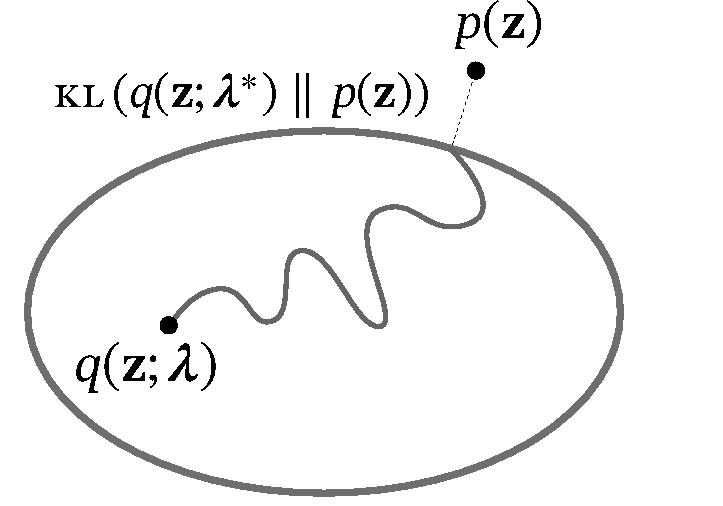
\includegraphics[height=0.2\paperheight]{fig/vi-cartoon.pdf}
  \caption[Variational inference cartoon]{
  \textbf{Variational inference finds the member of the variational family closest to the target distribution.} The oval in the cartoon represents the space of variational approximations $q(\mbz; \mblambda)$, and the goal of \acrlong{vi} is to find variational parameters $\mblambda^*$ that yield an approximation close to the target probability model $p(\mbz)$. One way to measure the distance between a variational approximation and the target probability distribution is with the \gls{kl} divergence.}
  \label{fig:vi-cartoon}
\end{figure}